\section{Reconstruction for VLA Observations}

Compressed Sensing Reconstruction used on two different tasks:
\begin{itemize}
	\item Center detection on sunburst data
	\item Reconstruction from incomplete measurements of Supernova Remnant G55
\end{itemize}

Two different problems. One is the 

Structure potentially smaller than the primary beam.



\subsection{Sunburst Center Detection}

Event date.

Sub- Primary Beam.
CS Objective Function

Figure: Dirty Map Peak, CLEAN, Single Peak Clean, Single Peak CS Reconstruction

\begin{figure}
	
\end{figure}

Wider Variance




\subsection{Reconstruction of Supernova Remnant G55}
\begin{figure}[h]
	\centering
	\begin{subfigure}[b]{0.45\linewidth}
		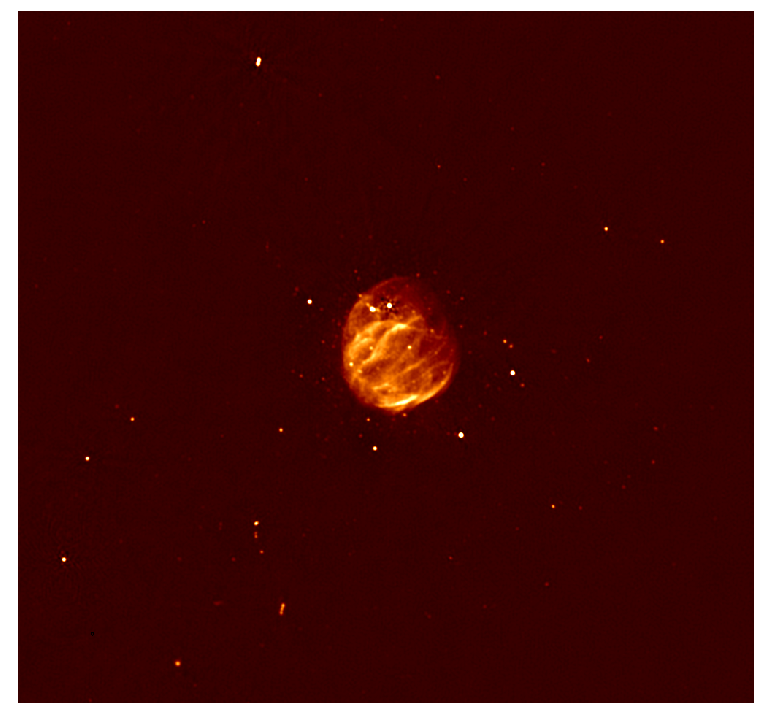
\includegraphics[width=\linewidth, trim={230px 210px 225px 200px}, clip]{./chapters/05.results/pic_G55_7.png}
		\caption{Reconstruction by NRAO.  Source:\cite{nraoG55}}
		\label{results:g55:nrao:rec}
	\end{subfigure}
	\begin{subfigure}[b]{0.45\linewidth}
		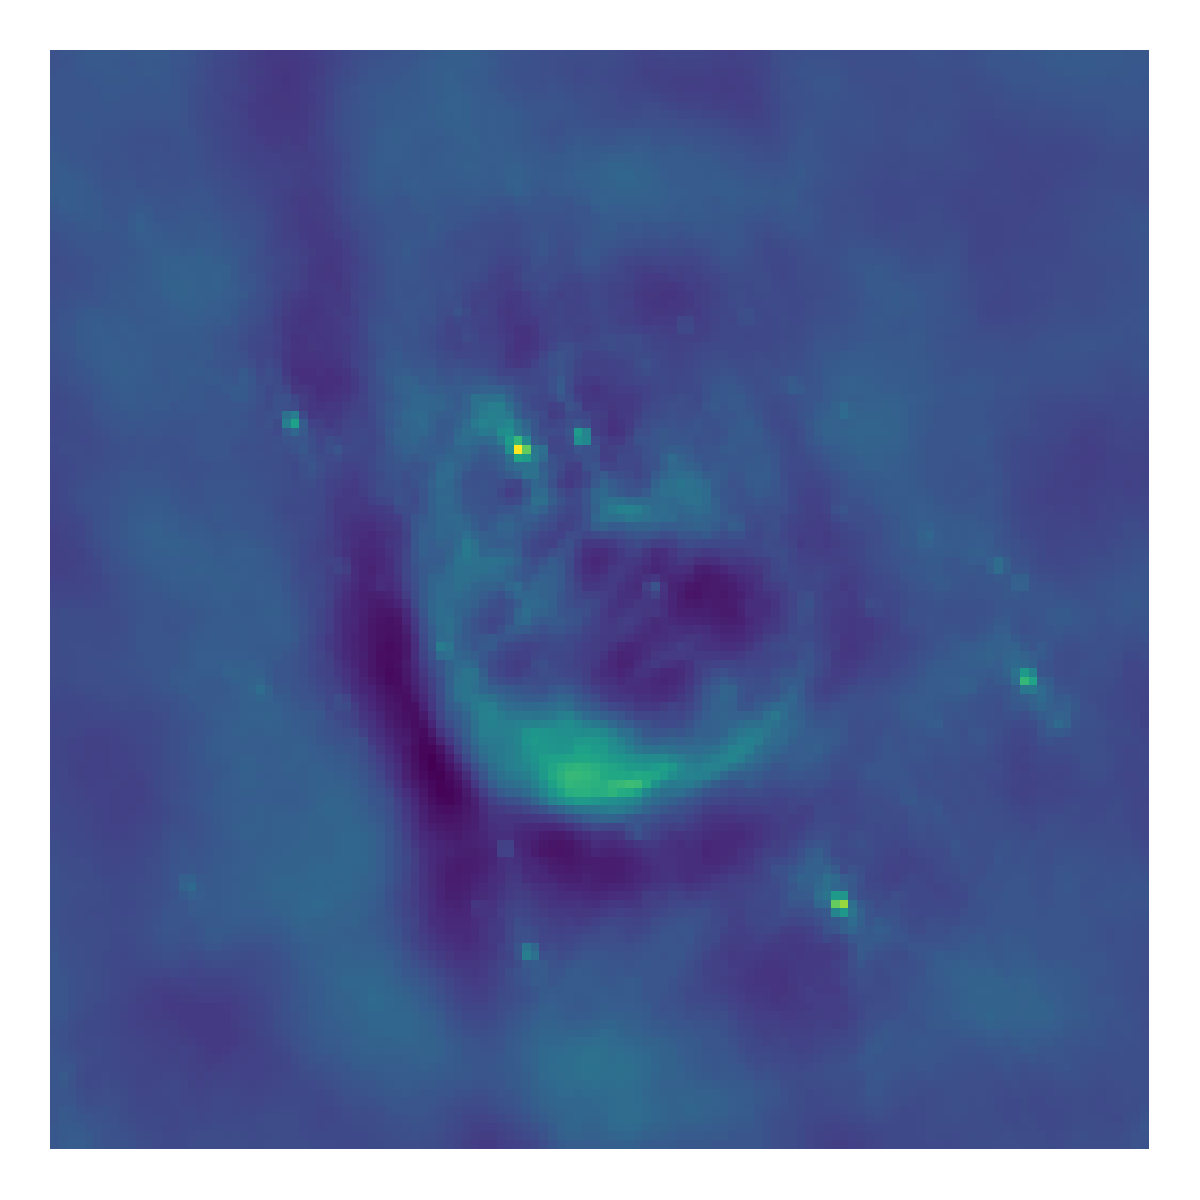
\includegraphics[width=\linewidth, trim={18px 19px 18px 18px}, clip]{./chapters/05.results/g55/raw_image.png}
		\caption{Dirty Image}
		\label{results:g55:nrao:dirty}
	\end{subfigure}
	\caption{SNR G55 source observed by VLA.}
	\label{results:g55:nrao}
\end{figure}

Data from the supernova remnant G55 are publicly available through the CASA imaging tutorial\cite{casaImagingGuide}. It is a 10 second calibrated observation by VLA. \ref{results:g55:nrao} is the dirty image from the 10 second observation. The full dataset contains 8 hours worth of data, which is not readily available. It is unknown if reconstruction \ref{results:g55:nrao:rec} was created with the full 8 hours or with another observation. The deconvolution algorithm is also unknown. For this project, the reconstructed image is assumed to show the true image of the sky.

The true image \ref{results:g55:nrao} has an "egg shaped" supernova remnant with a number of strong and faint point sources. Several tasks: Point Source detection and modelling of extended emissions. Point Sources inside extended emissions. The ideal Prior would

The dirty image\ref{results:g55:nrao:dirty} is of course corrupted by a point spread function, but it is not the only effect: There is negative "trench" striking through the image as well as brighter regions around the remnant.

Small field of View imaging was employed, even though this task is more a wide field imaging problem. It makes it harder for the deconvolution algorithms.

Several Priors were used with the an analysis objective and Gurobi as the optimizer.
Simple Priors


CLEAN algorithm, parameters were used from the CASA imaging tutorial. 

All algorithms constrain the model image to be non-negative. Physical plausible and shown to produce better results on synthetic data\cite{mcewen2011compressed}

Each Prior has a $\lambda$, it changes for each prior. The Miller\cite{miller1970least} $\lambda$ estimation was used and is shown in equation \eqref{results:eq:miller}. For the estimation an approximation of the solution $x$ is needed. In this project, the deconvolution was calculated without regularization and used to estimate the $\lambda$ parameter for each prior.

\begin{equation}\label{results:eq:miller}
	\lambda = e / E
\end{equation}

two figures, one with all reconstructed images for all algorithms. A cut through the image showing the intensity profile.

\begin{figure}[h]
	\centering
	\begin{subfigure}[b]{0.24\linewidth}
		\centering{Dirty Image}
		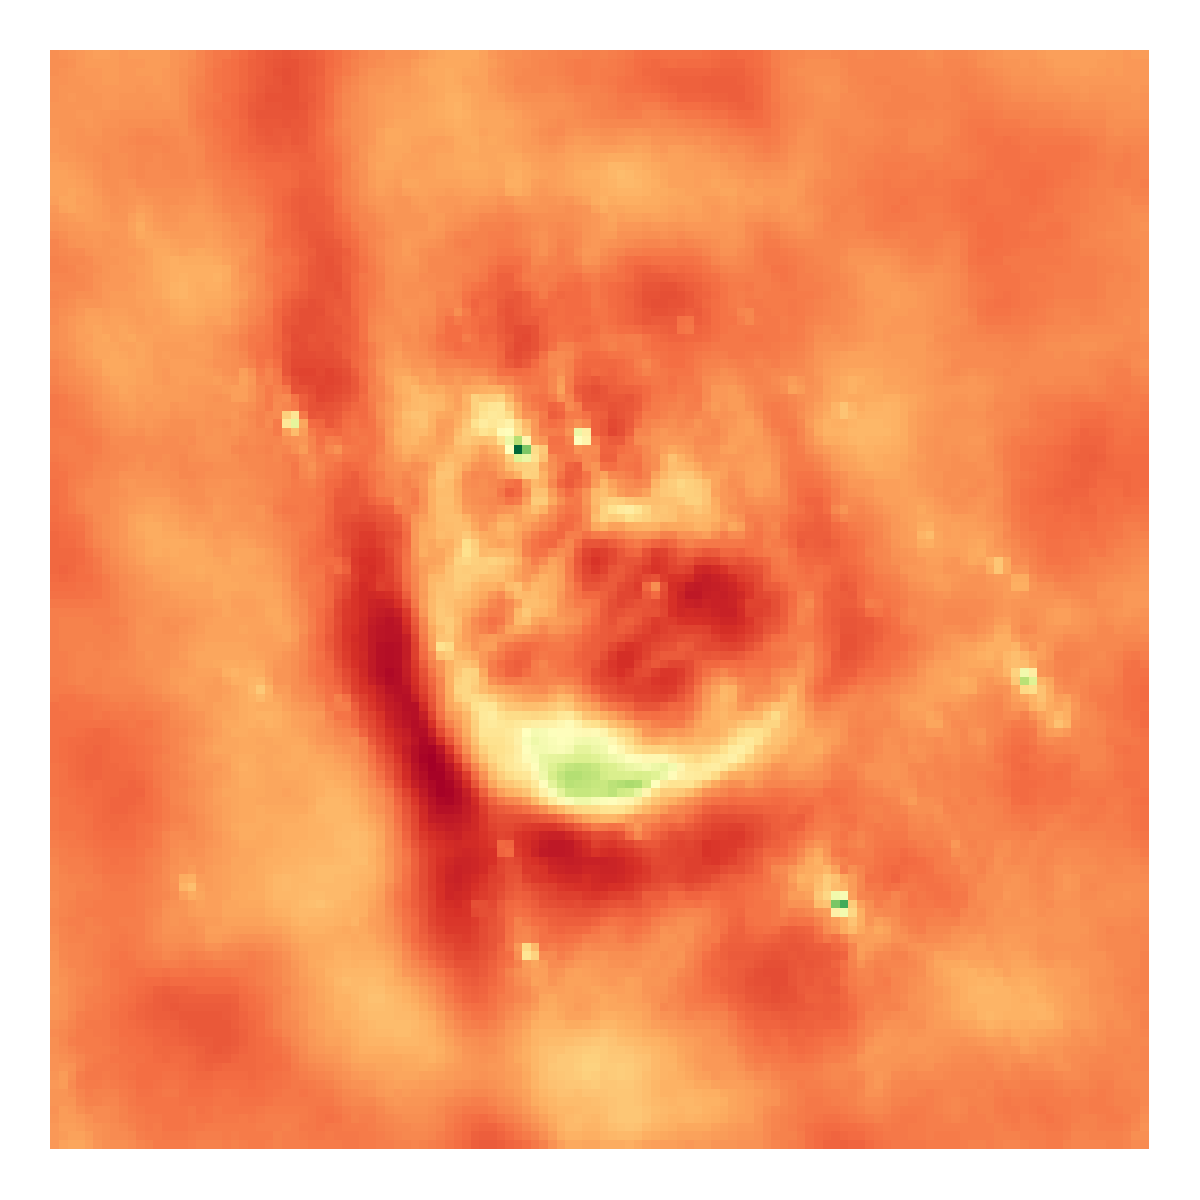
\includegraphics[width=\linewidth, trim={18px 19px 18px 18px}, clip]{./chapters/05.results/g55/raw_model.png}
	\end{subfigure}
	\begin{subfigure}[b]{0.24\linewidth}
		\centering{CLEAN}
		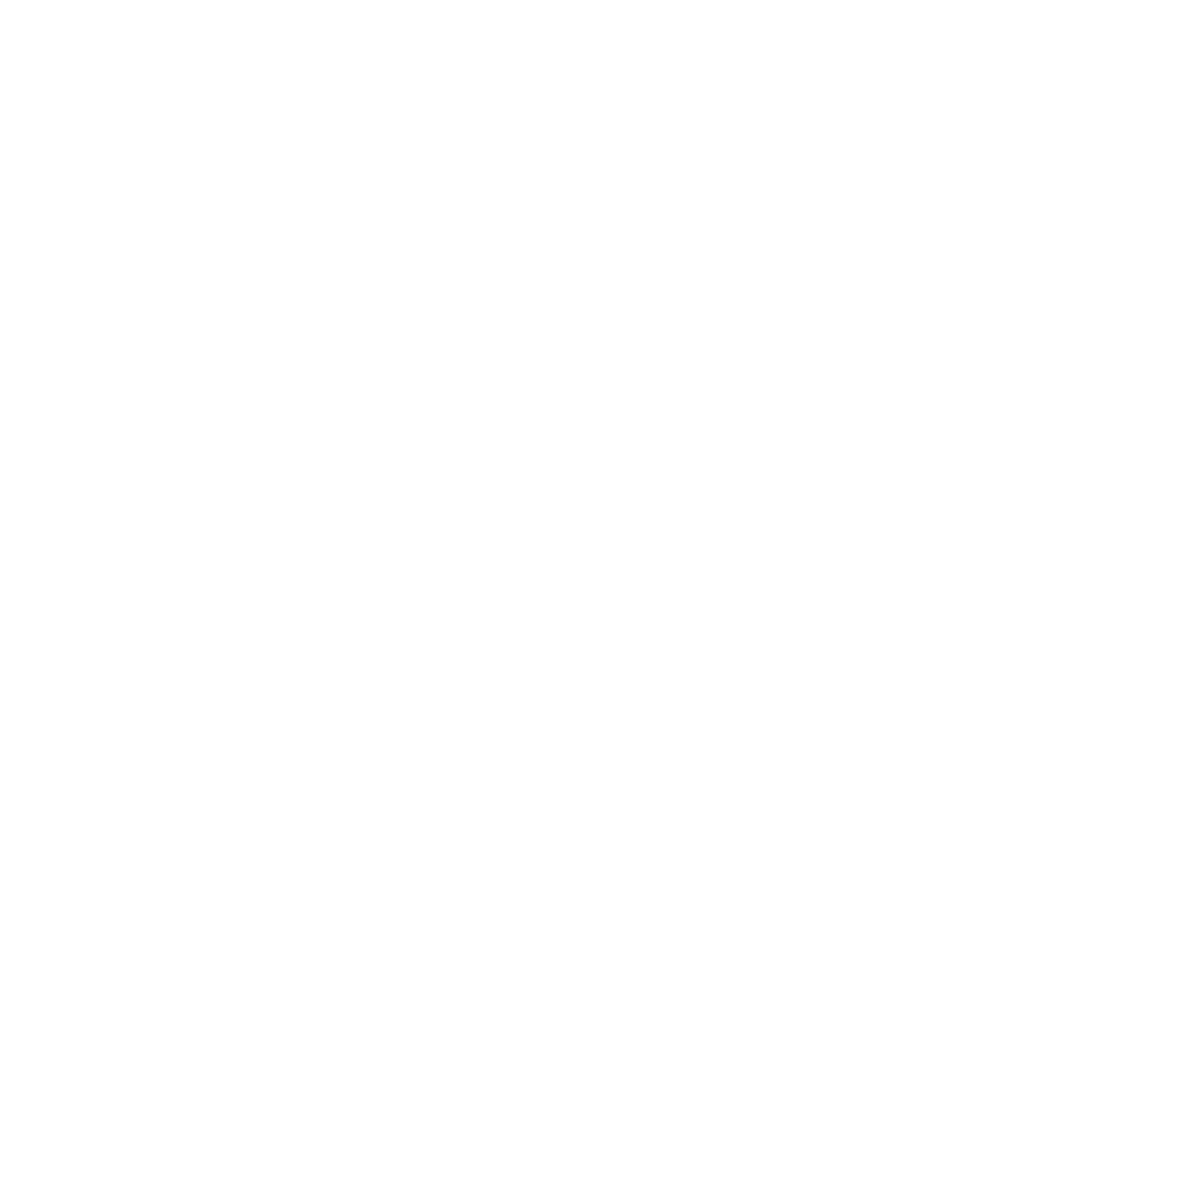
\includegraphics[width=\linewidth, trim={18px 19px 18px 18px}, clip]{./chapters/05.results/g55/clean_model.png}
	\end{subfigure}
	\begin{subfigure}[b]{0.24\linewidth}
		\centering{No Regularization}
		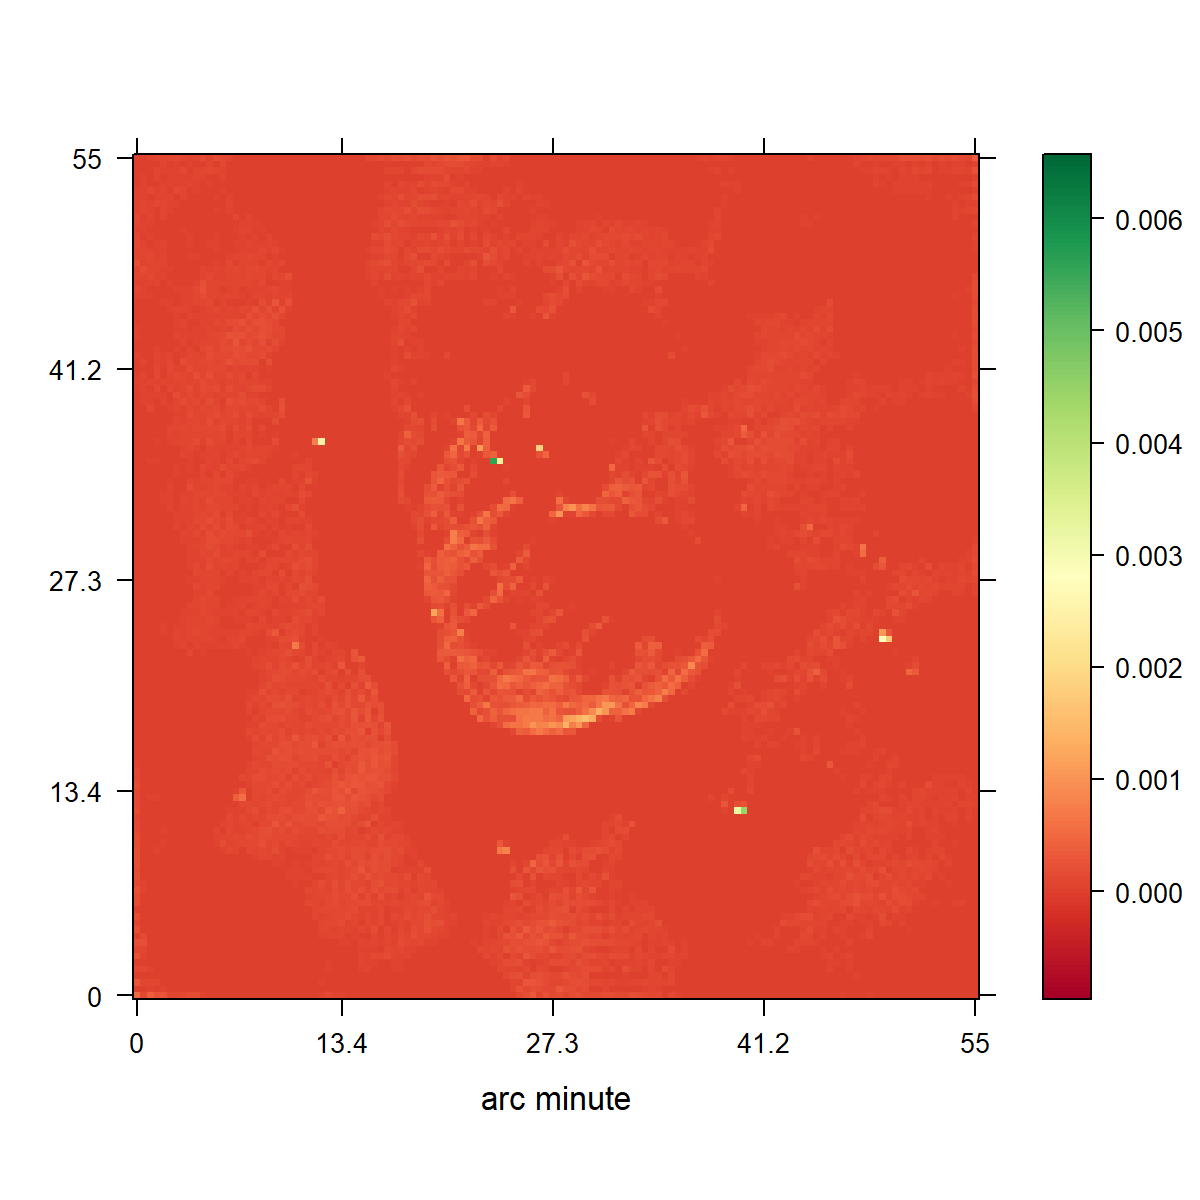
\includegraphics[width=\linewidth, trim={18px 19px 18px 18px}, clip]{./chapters/05.results/g55/positive_deconv_model.png}
	\end{subfigure}
	\begin{subfigure}[b]{0.24\linewidth}
		\centering{L1}
		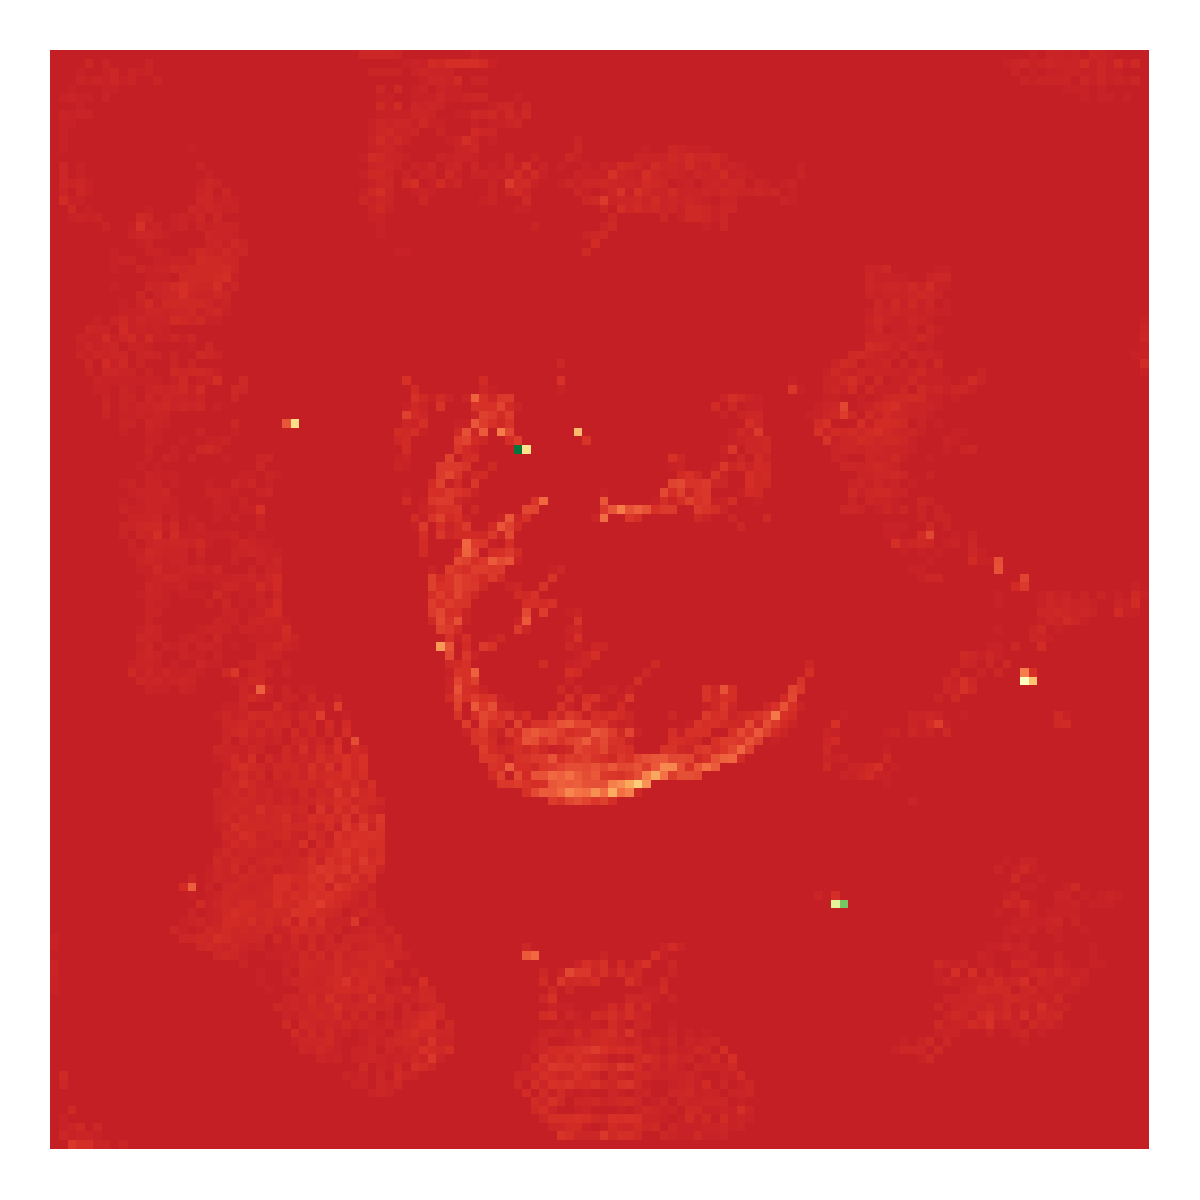
\includegraphics[width=\linewidth, trim={18px 19px 18px 18px}, clip]{./chapters/05.results/g55/L1_model.png}
	\end{subfigure}
	
	\begin{subfigure}[b]{0.24\linewidth}
		\vspace{10pt}
		\centering{L2}
		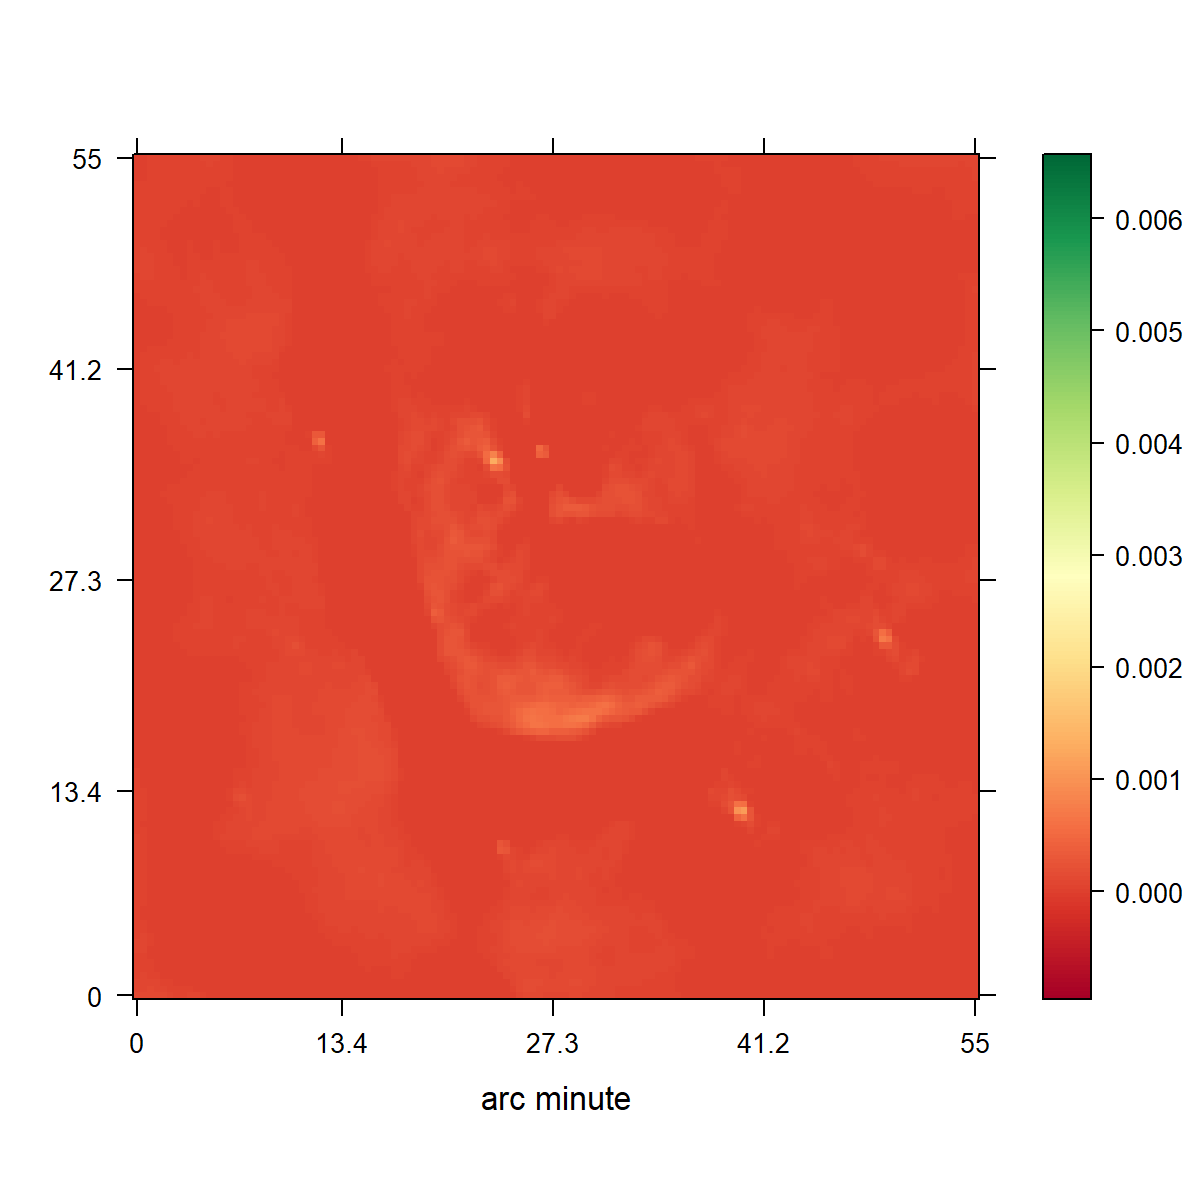
\includegraphics[width=\linewidth, trim={18px 19px 18px 18px}, clip]{./chapters/05.results/g55/L2_model.png}
	\end{subfigure}
	\begin{subfigure}[b]{0.24\linewidth}
		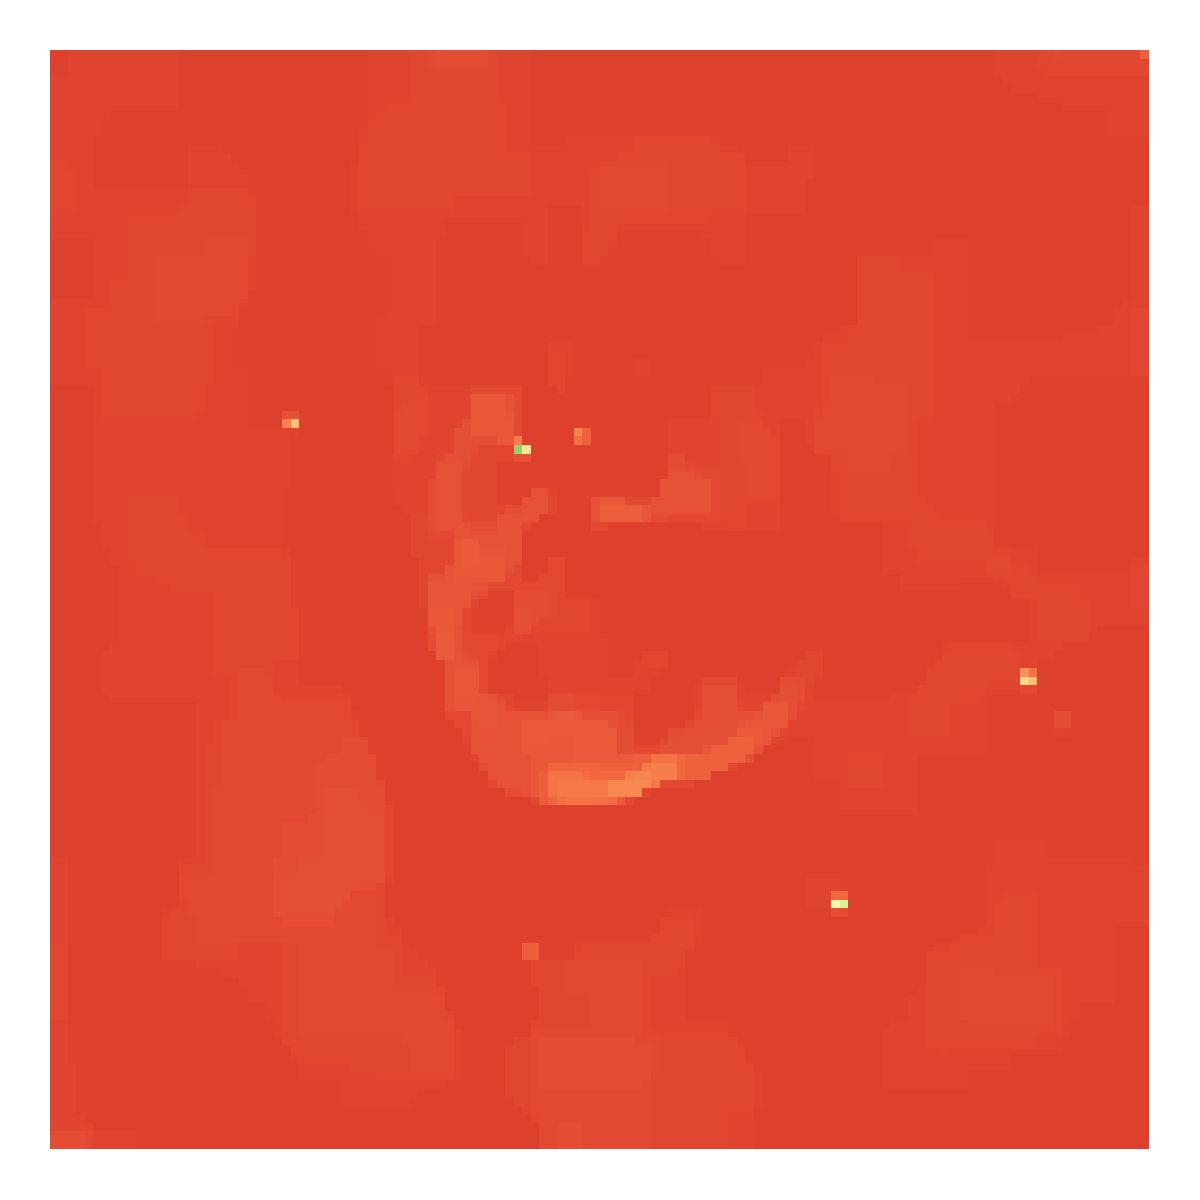
\includegraphics[width=\linewidth, trim={18px 19px 18px 18px}, clip]{./chapters/05.results/g55/TV_model.png}
	\end{subfigure}
	\begin{subfigure}[b]{0.24\linewidth}
		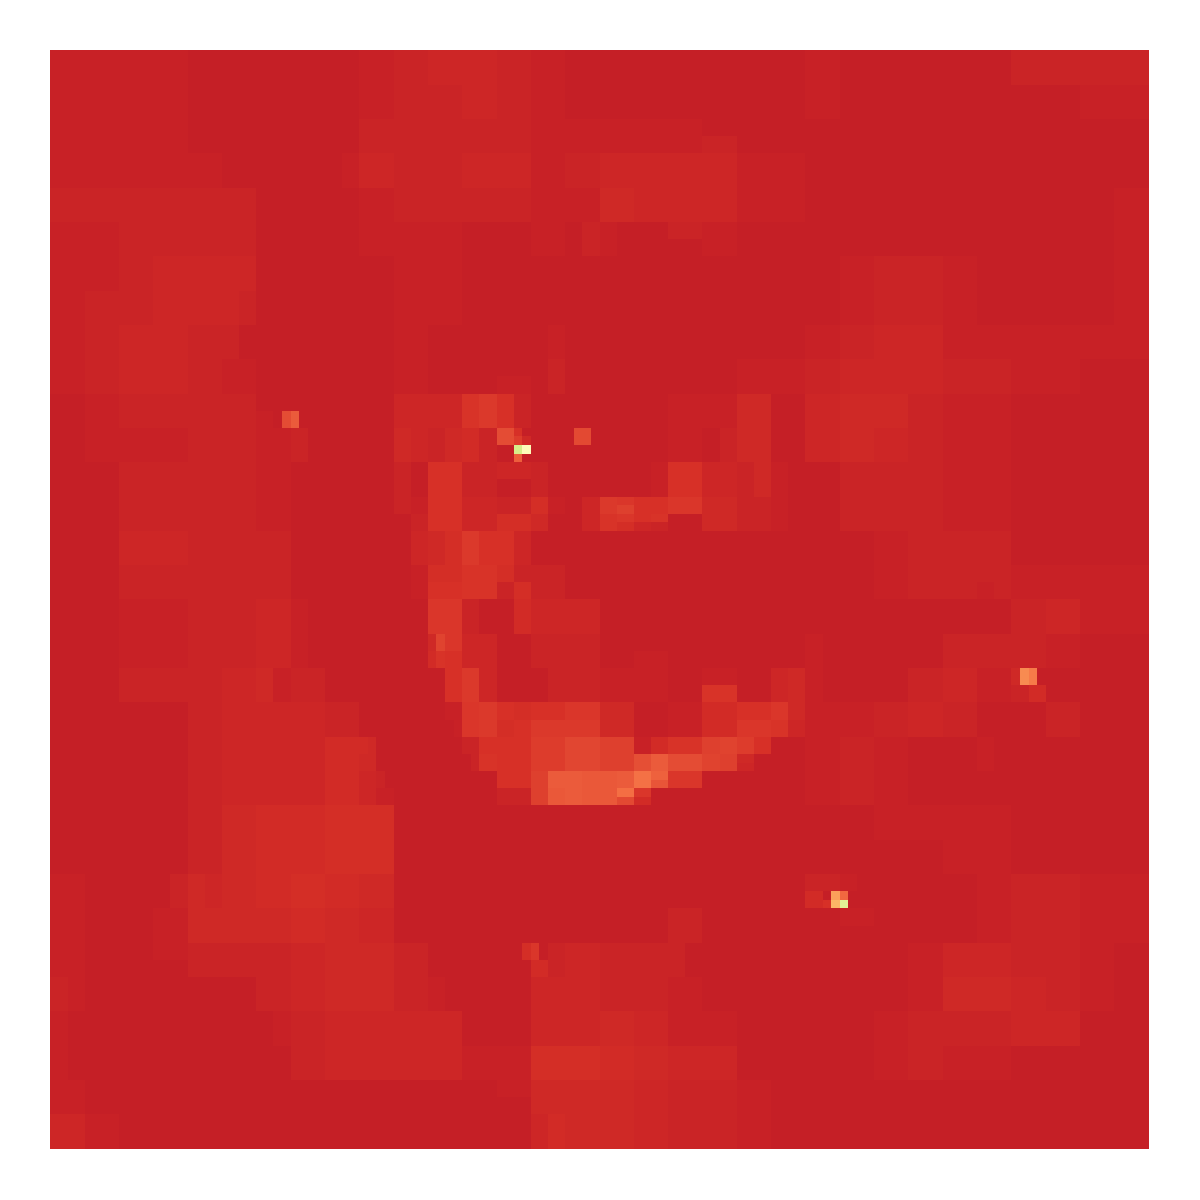
\includegraphics[width=\linewidth, trim={18px 19px 18px 18px}, clip]{./chapters/05.results/g55/haar_model.png}
	\end{subfigure}
	\begin{subfigure}[b]{0.24\linewidth}
		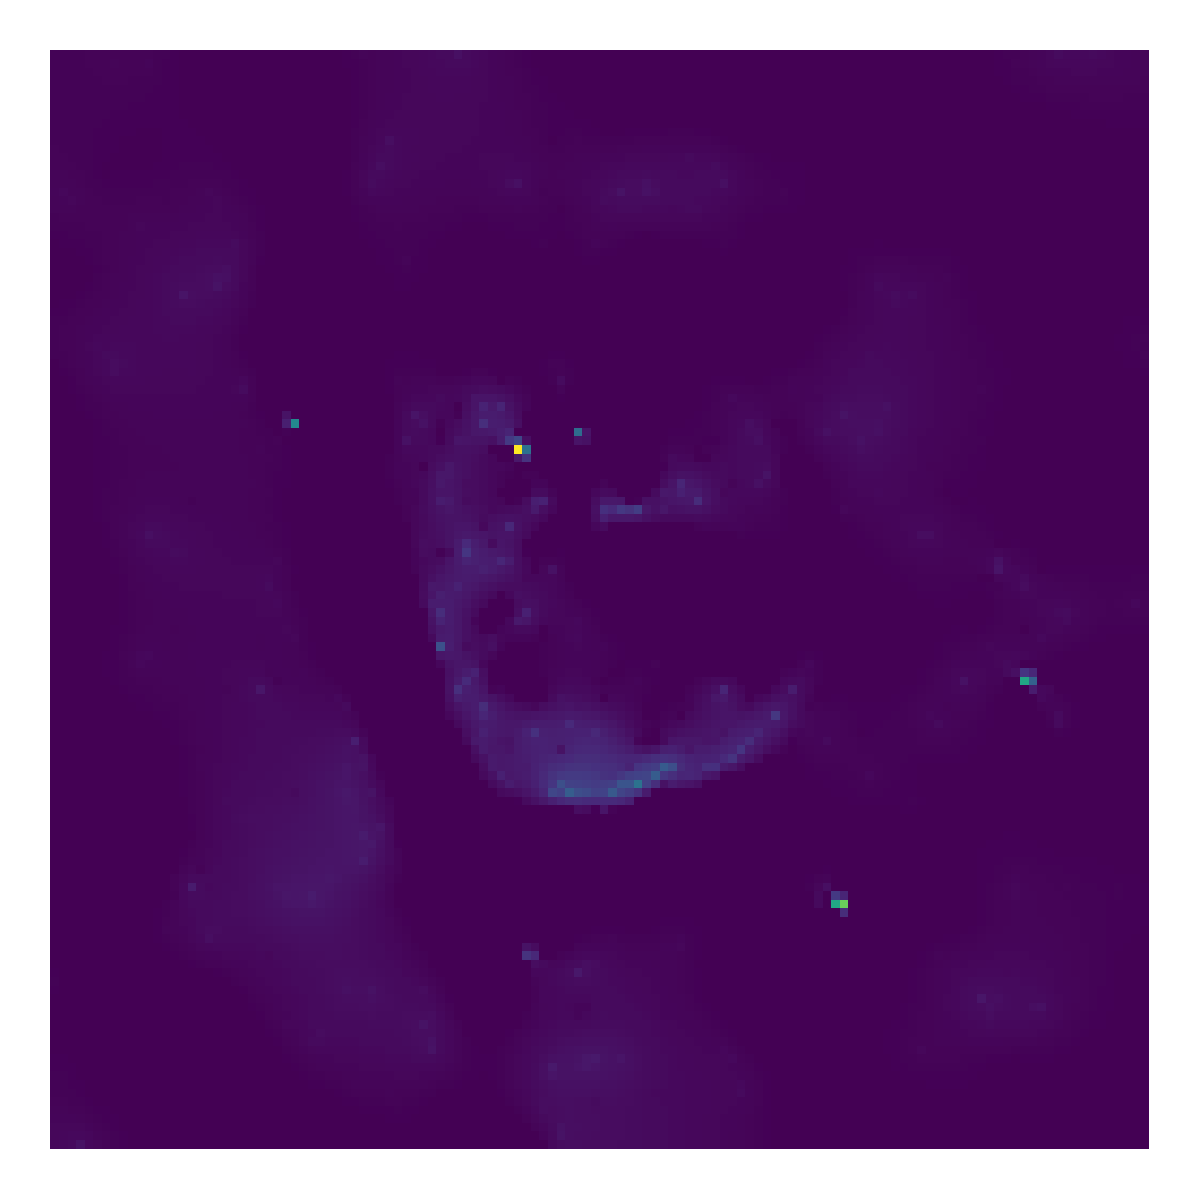
\includegraphics[width=\linewidth, trim={18px 19px 18px 18px}, clip]{./chapters/05.results/g55/starlets3_model.png}
	\end{subfigure}
\end{figure}

\begin{figure}
	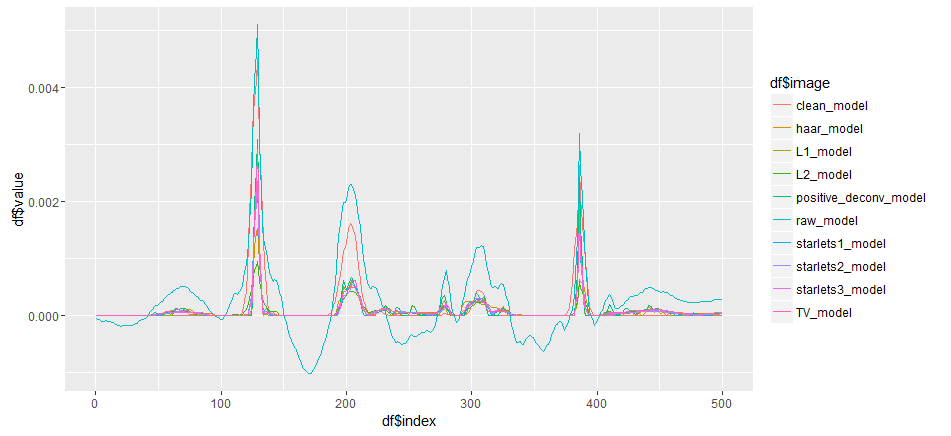
\includegraphics[width=\linewidth, trim={18px 19px 18px 18px}, clip]{./chapters/05.results/comparison_temp.png}
\end{figure}

CLEAN: Detects the brightest point sources. But only finds part of the extended emission. Limited resolution of the center. Not all point sources can be detected. CLEAN models the divet as a region of negative emission (parameters can be changed to stop this behaviour). in the profile large peaks but also wide.  

No Regularization: Detects the Egghead of the Remnant. Detects point sources in the fake extended emissions. The center has more details than clean. 
The non-negative Constraint stops the CS algorithms. 

L1: There is no visible difference between L1 and no regularization. Interaction with the miller lambda estimation. Extended emissions are not forced to be connected: the fake emissions have "holes" that are not plausible. Rocky ride in the profile.

L2: Forces the extended emissions to be more plausible, more details visible in the center. L2 also forces the point sources to be [lower and wider]. In the profile at around X shows more details in extended emissions.

\textbf{L1+L2}: Since L1 does a good job for point sources and L2 finds high-resolved details in extended sources, why does one not combine both? 
idea to combine both regularizations, get the best from both worlds. Flexibility of CS allows this prior. Tradeoff between point sources and extended. How to chose the tradeoff is not trivial, here it was assumed to be  equal. In this example, all pixels are very close to zero (Maximum: 0.0076 in Dirty Image), Miller lambda estimation is dominated by the L1 term while the L2 term gets neglected. The larger the values in the dirty image, the more L2 dominates over L1. Combination is not trivial.

Total Variation: Simple prior that was used in Image denoising. Reduces the gradient over the whole image. [It tries to have as few changes in the image as possible.] The reconstructed image shows both extended emissions and point sources. It has trouble with point sources inside extended emissions. In this case it cuts off the point source and the peak in image \ref{} is not here.

Starlets: A more sophisticated try at combining both. 





[No free lunch theorem.] The regularization decides what is noise and what is true. Search for regularization that finds the true image in every observation. CS is flexible and allows for a combination of regularization.

starlets finds a lot of smaller point sources, but they do

Problem with memory, $x \star PSF$ gets modeled as a vector matrix multiplication $Px$. The image $x$ and $PSF$ with dimensions of $128 * 128$, result in a matrix of size $128^2 * 128^2$. The memory requirement scales quadratic with the number of pixels. 
